\documentclass[11pt,a4paper]{article}

\usepackage[utf8]{inputenc}
\usepackage[T1]{fontenc}
\usepackage[margin=2.4cm]{geometry}
\usepackage{graphicx}
\usepackage{booktabs}
\usepackage{tabularx}
\usepackage{array}
\usepackage{float}
\usepackage{caption}
\usepackage{enumitem}
\usepackage{xcolor}
\usepackage{seqsplit}
\usepackage{tikz}
\usetikzlibrary{positioning,arrows.meta}
\usepackage[colorlinks=true,linkcolor=blue!50!black,urlcolor=blue!50!black]{hyperref}

% Charts are found either in the same folder (Overleaf) or in ../eda (inside the repository)
\graphicspath{{eda/}{../eda/}{./}}

\setlist{leftmargin=*,itemsep=2pt,topsep=3pt}
\captionsetup{font=small,labelfont=bf}
\newcommand{\file}[1]{\texttt{#1}}
\setlength{\emergencystretch}{3em}
\newcolumntype{R}{>{\raggedleft\arraybackslash}X}

\title{\textbf{SpillThePaper}\\[2pt]\large Deliverable 1: Problem Definition and Data Foundations\\[2pt]\normalsize AI Course Project, Track A (Application Development)}
\author{Minahil Basalat (24L-3082)\\ Iman Abid (24L-0707)\\ Khadija Rao (24L-3042)\\[4pt] FAST-NUCES}
\date{October 2026}

\begin{document}
\maketitle

\begin{abstract}
SpillThePaper is a Track~A project that will eventually turn historical university examination papers into a tentative, structured prediction of an upcoming paper and into personalised practice. This report covers only Deliverable~1: the problem definition (Phase~1) and the data acquisition and preprocessing foundation (Phase~2). We collected 3{,}567 exam-paper and course-outline files from a public student-maintained archive using a reproducible, configuration-driven pipeline; extracted text; built a structured table of 3{,}443 exam papers; handled missing values, duplicates and outliers; documented an encoding and scaling strategy; and produced exploratory charts. No prediction model has been trained yet. All numbers in this report come from executions of the scripts in the project repository.
\end{abstract}

\tableofcontents
\newpage

%=====================================================================
\section{Introduction}
Students at FAST-NUCES often have access to many past mid-term, final and quiz papers, but the collection is large, unstructured and inconsistent. SpillThePaper aims to turn this archive into evidence-based exam preparation. The complete system (Phases~3--6) will analyse patterns, estimate how likely syllabus areas are to appear, generate a tentative paper, and personalise follow-up practice.

\paragraph{Scope of this report.} Deliverable~1 requires (i) a problem statement, target audience and AI justification, and (ii) evidence of data collection, cleaning scripts for missing values, duplicates and outliers, a feature strategy (normalisation, scaling, encoding), and initial exploratory data analysis. We deliberately do \emph{not} implement the prediction engine, paper generator, personalisation, user interface or deployment here. The code is in the project repository \url{https://github.com/Minahilbasalat/SpillThePaper}, in the folder \file{data scripts/}.

\begin{table}[H]
\centering
\caption{Deliverable 1 requirements and where this report covers them.}
\label{tab:map}
\begin{tabularx}{\linewidth}{>{\raggedright\arraybackslash}Xl}
\toprule
Requirement & Section \\
\midrule
Problem statement (real-world pain point) & \ref{sec:problem} \\
Target audience & \ref{sec:audience} \\
AI justification (why ML rather than rule-based programming) & \ref{sec:ai} \\
Collection: evidence of data gathering & \ref{sec:collection} \\
Cleaning: missing values, duplicates, outliers & \ref{sec:missing}, \ref{sec:dups}, \ref{sec:outliers} \\
Feature strategy: normalisation, scaling, encoding & \ref{sec:features} \\
EDA charts of the raw data, including class distributions and feature correlations & \ref{sec:eda} (Figures~\ref{fig:class} and~\ref{fig:corr}) \\
Repository layout, \file{data scripts/} folder & Appendix~\ref{app:repo} \\
\bottomrule
\end{tabularx}
\end{table}

%=====================================================================
\section{Problem Definition}

\subsection{Problem Statement}
\label{sec:problem}
University students often have access to a large collection of past quizzes, mids, and finals, but deciding what to study from them can be difficult. At FAST, papers are available across different semesters and courses, but students usually have to review them manually and rely on guesswork, senior advice, or assumptions about what might appear again.

This creates several problems:
\begin{itemize}
  \item \textbf{Patterns are difficult to identify:} Students may miss recurring topics, question types, difficulty levels, and marks distributions when analyzing many papers manually.
  \item \textbf{Syllabi change over time:} A topic that appeared frequently in older papers may have been removed, reduced, or changed in the current syllabus, making older patterns less reliable.
  \item \textbf{Too many papers to study:} Although a large number of past papers are available, students often have limited preparation time and cannot realistically study all of them.
  \item \textbf{Risk of over-preparing predicted topics:} Focusing only on frequently repeated topics can leave students unprepared for less predictable areas of the syllabus.
  \item \textbf{Preparation is not personalized:} Students have different strengths and weaknesses, but traditional past-paper practice does not identify which areas an individual student needs to improve.
  \item \textbf{Time management is overlooked:} Many students struggle to complete a one-hour exam even after practicing, but they may not have a realistic way to assess their speed and time management before the actual exam.
\end{itemize}
Therefore, there is a need for a system that can analyze historical papers and current course information to identify useful patterns and provide focused, realistic exam preparation without relying entirely on manual analysis or guesswork.

\subsection{Target Audience}
\label{sec:audience}
\begin{itemize}
  \item \textbf{Primary users:} FAST-NUCES undergraduate students (starting with CS/AI/SE-type courses) preparing for mids, finals and quizzes.
  \item \textbf{Courses supported:} those with enough historical papers to find patterns. Courses with very few papers will be flagged as low-confidence.
  \item \textbf{Secondary (future):} students who add their own subject, papers or the current course outline.
  \item \textbf{Not targeted:} students outside this exam culture, or courses with no past-paper history.
\end{itemize}

\subsection{AI Justification}
\label{sec:ai}
A simple rule such as ``if a topic appeared 5 times, predict it'' is easy to implement, but it is not sufficient for this problem because exam patterns depend on multiple changing factors:
\begin{enumerate}
  \item \textbf{The input is unstructured text.} Questions are extracted from PDFs and may use different wording for the same concept. NLP techniques are needed to identify topics and question types beyond simple keyword matching.
  \item \textbf{Multiple factors interact.} Frequency, recency, assessment type, marks, topic combinations, difficulty, and syllabus relevance can all affect a topic's importance. Their combined influence is difficult to capture using manually defined rules.
  \item \textbf{Exam patterns change over time.} Topics may become more or less relevant, syllabi can change, and question styles can shift. A learning-based approach can identify these changing patterns from historical data rather than relying on fixed rules.
  \item \textbf{Predictions are uncertain.} The system should estimate the likelihood of different topics and question types rather than making a simple yes/no decision. This allows the generated paper to include both high-probability and less predictable syllabus areas.
  \item \textbf{Syllabus matching requires semantic understanding.} Comparing questions from older papers with the current syllabus requires understanding similar concepts even when different words are used, making text similarity or embeddings more suitable than exact keyword matching.
  \item \textbf{Personalization requires learning from performance.} Identifying a student's weak areas from their answers and adapting future practice papers is a data-driven learning task that cannot be effectively handled through fixed rules alone.
\end{enumerate}
Therefore, Machine Learning and NLP provide the flexibility needed to learn patterns from historical exam data, adapt to changing trends, understand unstructured question text, and eventually support personalized preparation.

\paragraph{Scope note.} No model has been trained in Deliverable~1. This section explains why the full problem suits machine learning, and Phase~2 builds the data foundation for it. Our exploratory results already support two of the points above: papers differ strongly by assessment type, and data coverage differs strongly by subject and year (Section~\ref{sec:eda}).

%=====================================================================
\section{Data Acquisition}

\subsection{Data Source}
The data source is the public GitHub repository \emph{Academic-Time-Machine} (\url{https://github.com/saleha-muzammil/Academic-Time-Machine}), a student-maintained archive of past papers, course outlines, books and notes. All collection was pinned to commit \texttt{\seqsplit{e0e197577432957a5fad0f76d2ab92d78f48e1d8}}, so the exact snapshot can be re-collected. The archive is community contributed and not curated; Section~\ref{sec:limits} discusses what this means for data quality. We do not redistribute the raw files: they are downloaded by our scripts into a folder that is excluded from version control.

\subsection{Repository Structure and Issues Found}
We inspected the real structure before writing any code. The repository contains 8{,}562 files (Table~\ref{tab:repo}). The structure is \emph{not} uniform. Subject folders contain assessment folders (\emph{Quiz}, \emph{Mid-1}, \emph{Finals}\ldots), term folders (\emph{Spring 2022}), or loose files, sometimes in several patterns within one subject. Term and year appear in folder names, in file names (for example \emph{F22}), as ranges (\emph{2013-19}) or not at all.

\begin{table}[H]
\centering
\caption{Composition of the repository at the collected commit (eight most common file types).}
\label{tab:repo}
\begin{tabular}{lr}
\toprule
File type & Files \\
\midrule
.pdf & 4{,}901 \\
.docx & 571 \\
.jpg & 488 \\
.c & 401 \\
.java & 330 \\
.txt & 324 \\
.pptx & 285 \\
.cpp & 217 \\
\midrule
All files & 8{,}562 \\
\bottomrule
\end{tabular}
\end{table}

Problems identified before processing: inconsistent subject names (for example \texttt{OOP} and \texttt{Object Oriented Programming}); solutions stored beside papers; merged files that repeat individual papers; the same paper stored in several places; photographs and scanned PDFs instead of text PDFs; slides, code and assignments mixed with exam material; and many files without a year.

\paragraph{Professor information.} We investigated whether instructor information exists. File paths of papers and quizzes contain no reliable instructor name, and there is no mapping from quizzes to instructors. At least some course outlines contain an instructor name in their text, but outlines cannot be linked to individual quizzes. Professor-specific analysis is therefore \emph{not} supported by the current data and is listed as future work; no instructor information is used or reported.

\subsection{Collection Method}
\label{sec:collection}
Collection is implemented as three scripts that run in order (Figure~\ref{fig:pipeline}). Subject names are never hard-coded: rules live in configuration files (\path{config/filters.yaml}, \path{config/assessment_rules.yaml}), so adding a subject, semester or paper to the source archive requires adding data, not changing code.

\begin{figure}[H]
\centering
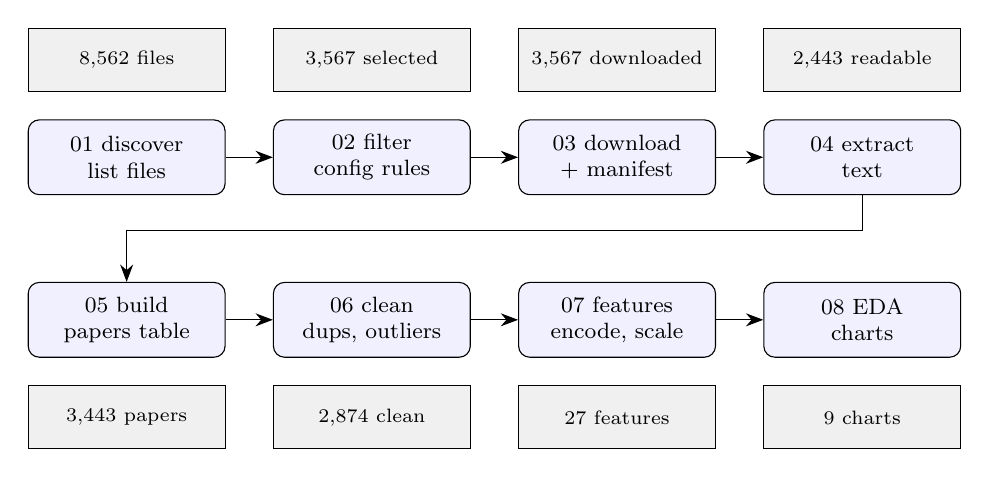
\begin{tikzpicture}[
  box/.style={rectangle,draw,rounded corners,align=center,minimum width=2.5cm,minimum height=0.95cm,font=\footnotesize,fill=blue!6},
  data/.style={rectangle,draw,align=center,minimum width=2.5cm,minimum height=0.8cm,font=\scriptsize,fill=gray!12},
  arr/.style={-{Stealth[length=2.2mm]}}]
  \node[box] (d1) {01 discover\\list files};
  \node[box,right=0.6cm of d1] (d2) {02 filter\\config rules};
  \node[box,right=0.6cm of d2] (d3) {03 download\\+ manifest};
  \node[box,right=0.6cm of d3] (d4) {04 extract\\text};
  \node[box,below=1.1cm of d1] (d5) {05 build\\papers table};
  \node[box,right=0.6cm of d5] (d6) {06 clean\\dups, outliers};
  \node[box,right=0.6cm of d6] (d7) {07 features\\encode, scale};
  \node[box,right=0.6cm of d7] (d8) {08 EDA\\charts};
  \draw[arr] (d1) -- (d2); \draw[arr] (d2) -- (d3); \draw[arr] (d3) -- (d4);
  \draw[arr] (d4.south) -- ++(0,-0.45) -| (d5.north);
  \draw[arr] (d5) -- (d6); \draw[arr] (d6) -- (d7); \draw[arr] (d7) -- (d8);
  \node[data,above=0.35cm of d1] {8{,}562 files};
  \node[data,above=0.35cm of d2] {3{,}567 selected};
  \node[data,above=0.35cm of d3] {3{,}567 downloaded};
  \node[data,above=0.35cm of d4] {2{,}443 readable};
  \node[data,below=0.35cm of d5] {3{,}443 papers};
  \node[data,below=0.35cm of d6] {2{,}874 clean};
  \node[data,below=0.35cm of d7] {27 features};
  \node[data,below=0.35cm of d8] {9 charts};
\end{tikzpicture}
\caption{Data pipeline for Deliverable~1. Numbers are file or row counts from the actual run. Raw downloads and extracted text are not stored in the repository.}
\label{fig:pipeline}
\end{figure}

\begin{enumerate}
  \item \textbf{Discover} (\file{01\_discover.py}): one request to the GitHub API returns the whole file tree and the commit identifier, with no paper downloaded.
  \item \textbf{Filter} (\file{02\_filter.py}): keeps quizzes, mids, finals and course outlines. Assessment type is read from the file name first, then from folder names from the deepest upward. Non-exam material (assignments, slides, lectures, notes) is skipped, and every excluded file is listed with its reason.
  \item \textbf{Download} (\file{03\_download.py}): downloads the selected files at the pinned commit, streams them to disk, can be stopped and resumed, and writes a manifest with the size and SHA-256 hash of every file.
\end{enumerate}

\subsection{Collection Evidence and Statistics}
Table~\ref{tab:collection} summarises the collection. All 3{,}567 selected files were downloaded with no failures; the manifest (\file{collection\_manifest.csv}) and logs (\file{logs/collection\_log.txt}) are stored in the repository as evidence. The script estimated a download size of about 2{,}418~MB; the largest single file was about 62~MB.

\begin{table}[H]
\centering
\caption{Results of filtering the 8{,}562 repository files.}
\label{tab:collection}
\begin{tabularx}{\linewidth}{Xr}
\toprule
\textbf{Selected files} & \textbf{3{,}567} \\
\quad quizzes & 1{,}400 \\
\quad mids & 1{,}215 \\
\quad finals & 819 \\
\quad course outlines & 124 \\
\quad exam papers with type not written in the path (\emph{exam\_unspecified}) & 9 \\
\quad by format: PDF 2{,}911; Word 312; photographs (jpg/jpeg/png) 344 & \\
\midrule
\textbf{Excluded files} & \textbf{4{,}995} \\
\quad file type not allowed (code, slides, text, \ldots) & 1{,}956 \\
\quad top-level books and notes folder & 1{,}184 \\
\quad file name is clearly not an exam (assignment, slides, \ldots) & 725 \\
\quad inside a non-exam folder & 607 \\
\quad no quiz/mid/final keyword in name or folders & 523 \\
\midrule
Distinct subject folder names among selected files & 142 \\
Files downloaded successfully & 3{,}567 \\
\bottomrule
\end{tabularx}
\end{table}

\subsection{Challenges Encountered}
\begin{itemize}
  \item \textbf{Irregular structure:} no single parsing rule fits all folders, so classification uses prioritised, configurable patterns. After reviewing samples we corrected several rules (for example, so that a folder called ``Material'' does not hide a ``Mid-2'' folder inside it).
  \item \textbf{Memory error during download:} the first download script loaded each file fully into memory and crashed on a large file. We rewrote it to stream to disk in chunks, write to a temporary file, and skip files above a size limit.
  \item \textbf{Scanned papers:} about one third of files contain no extractable text (Section~\ref{sec:extraction}).
\end{itemize}

%=====================================================================
\section{Data Preprocessing}

\subsection{Text Extraction}
\label{sec:extraction}
We tested two PDF readers on eight sample papers. They gave similar results on seven; on one AI-lab quiz the \texttt{pypdf} library ran words together and returned 7 words where PyMuPDF returned 135 correctly spaced words. We therefore use PyMuPDF for PDFs and \texttt{python-docx} for Word files. PDFs with almost no text per page, and photographs, are flagged \emph{needs OCR} rather than processed, because OCR would add software and hours of computation that Deliverable~1 does not require. Table~\ref{tab:extraction} shows the result.

\begin{table}[H]
\centering
\caption{Text extraction results for the 3{,}567 downloaded files.}
\label{tab:extraction}
\begin{tabular}{lr}
\toprule
Method / result & Files \\
\midrule
PDF with text (PyMuPDF) & 2{,}132 \\
Word document (python-docx) & 311 \\
No readable text, flagged for OCR (scanned PDF or photograph) & 1{,}123 \\
Could not be opened (corrupt Word file) & 1 \\
\bottomrule
\end{tabular}
\end{table}

\subsection{Building the Papers Table}
The script \file{05\_build\_papers.py} converts the 3{,}567 files into two tables: 3{,}443 exam papers and 124 course outlines. It distinguishes three kinds of columns:
\begin{itemize}
  \item \textbf{Raw} (from path and file name): subject folder, assessment type, assessment number (for example Mid~1), term, year, class section, and syllabus tag when written.
  \item \textbf{Extracted} (from the text): total marks, an estimated question count, page and word counts, and the year from the paper header when the path has none.
  \item \textbf{Derived} (our flags): solution, merged-compilation, retake, and lab-subject flags, a cleaned subject name, and a readable-text flag.
\end{itemize}
Subject names are cleaned with a configuration file of mappings (for example merging \texttt{OOP} with \texttt{Object Oriented Programming}). We only merged names that clearly denote the same course, and kept laboratory courses separate from theory courses. Fields that need NLP (topic, subtopic, difficulty, question type) are \emph{not} available at this stage and are not pretended to exist.

\begin{table}[H]
\centering
\caption{Where the year and term of the 3{,}443 papers came from.}
\label{tab:termsource}
\begin{tabular}{lr}
\toprule
Source & Papers \\
\midrule
Season and year found in the path or file name & 2{,}015 \\
Year only found in the path (no season) & 179 \\
Recovered from the paper header text & 666 \\
Not found & 583 \\
\bottomrule
\end{tabular}
\end{table}

Reading the header recovered the year for 666 papers that the path did not describe; without this step the year would be missing for about 36\% of papers instead of 17\%.

\subsection{Missing Values}
\label{sec:missing}
Table~\ref{tab:missing} reports missing values before cleaning (Figure~\ref{fig:missing} shows the same data). Our policy is to \emph{never delete a row only because a field is missing}. Instead we (i) recover values from a second source where possible (header text for year); (ii) treat impossible values as missing (the check for total marks outside 1--200 found no such value); (iii) keep other gaps as missing and record them; and (iv) exclude a paper from text analysis only, not from metadata analysis, when it has no readable text. Imputation for modelling is described in Section~\ref{sec:features}.

\begin{table}[H]
\centering
\caption{Missing values among the 3{,}443 exam papers (before cleaning).}
\label{tab:missing}
\begin{tabular}{lrrr}
\toprule
Field & Missing & Out of & \% \\
\midrule
Subject (file in repository root) & 2 & 3{,}443 & 0.1 \\
Assessment type not written (\emph{exam\_unspecified}) & 9 & 3{,}443 & 0.3 \\
Year & 583 & 3{,}443 & 16.9 \\
Term (season), among papers with a year & 219 & 2{,}860 & 7.7 \\
Assessment number, among mids and quizzes & 374 & 2{,}615 & 14.3 \\
Class section & 3{,}268 & 3{,}443 & 94.9 \\
Readable text & 1{,}123 & 3{,}443 & 32.6 \\
Total marks, among papers with text & 852 & 2{,}320 & 36.7 \\
Estimated question count, among papers with text & 732 & 2{,}320 & 31.6 \\
\bottomrule
\end{tabular}
\end{table}

\subsection{Duplicate Handling}
\label{sec:dups}
Duplicates matter because the same questions would be counted twice in any later frequency analysis. Four rules are applied in order; a paper is excluded by the first rule that matches, and every exclusion is recorded with its reason and the file it duplicates.
\begin{enumerate}
  \item \textbf{Exact duplicate:} identical file content (same SHA-256 hash); one copy is kept.
  \item \textbf{Same-text duplicate:} identical text after removing case, spacing and punctuation (texts under 200 characters are not compared); one copy is kept.
  \item \textbf{Merged compilation:} files such as ``all finals merged'', which repeat individual papers and cannot be tied to one year.
  \item \textbf{Solution companion:} a solution file when the same paper (same subject, type, number, year, term and section) also exists without a solution.
\end{enumerate}
Table~\ref{tab:funnel} and Figure~\ref{fig:funnel} show the effect: 3{,}443 papers became 2{,}874 (a reduction of 16.5\%), of which 1{,}823 have readable text. Solution files that cannot be paired with a plain paper are kept, because they are often the only copy (a single PDF containing both paper and answers); they remain flagged so that later phases can treat their content carefully.

\begin{table}[H]
\centering
\caption{Papers remaining after each cleaning step.}
\label{tab:funnel}
\begin{tabular}{lrr}
\toprule
Step & Excluded & Remaining \\
\midrule
Start & -- & 3{,}443 \\
Exact duplicates & 160 & 3{,}283 \\
Same-text duplicates & 49 & 3{,}234 \\
Merged compilations & 51 & 3{,}183 \\
Solution companions & 309 & 2{,}874 \\
\bottomrule
\end{tabular}
\end{table}

\subsection{Outlier Handling}
\label{sec:outliers}
Outlier detection is applied \emph{only to numeric columns}: page count, word count, total marks and estimated question count. We use the interquartile-range rule (values beyond 1.5 IQR from the quartiles), computed separately for each assessment type, because a normal final is much longer than a normal quiz. Outliers are \emph{flagged but not removed}, since a long paper may be legitimate. On the 2{,}874 clean papers, 94 are flagged for pages, 73 for words, 47 for total marks and 84 for question count, and 257 papers (8.9\%) are flagged on at least one column. Text is never subjected to statistical outlier detection.

\subsection{Feature Strategy: Encoding, Scaling and Normalisation}
\label{sec:features}
We apply a transformation only where it is meaningful and document why not otherwise (Table~\ref{tab:features}). The resulting table (\file{features.csv}) has 2{,}874 rows and 27 columns. Plain pandas is used, so every step is transparent.

\begin{table}[H]
\centering
\caption{Feature strategy.}
\label{tab:features}
\small
\begin{tabularx}{\linewidth}{>{\raggedright\arraybackslash}p{3.1cm}>{\raggedright\arraybackslash}p{2.6cm}>{\raggedright\arraybackslash}X}
\toprule
Feature & Type & Treatment and reason \\
\midrule
Assessment type, term & Categorical (nominal) & One-hot encoding: few categories, no order. ``Unknown'' term is its own category so no rows are dropped. \\
Subject & Categorical, 131 values & Not one-hot: many subjects have few papers, so it would create mostly empty columns. The name is kept for grouping and a paper-count (frequency) feature is added. Richer encodings are deferred to Phase~3. \\
Solution, retake, lab, has-text, outlier flags & Binary & Stored as 0/1. \\
Year & Numeric (time) & Min--max scaled to $[0,1]$ as a recency value. Unknown years (525 papers) stay missing with a flag, because a year cannot be honestly guessed. \\
Pages, words, total marks, question count, subject paper count & Numeric counts & Skewness was 4.5, 2.53, 1.04, 2.58 and 1.45, so all use a $\log(1+x)$ transform followed by z-score scaling. Missing values (pages 226, words 1{,}051, total marks 1{,}674, question count 1{,}630 papers) are filled with the median of the same assessment type, and a missing-value flag is added. \\
Paper text & Text & No scaling or normalisation now (numeric scaling is meaningless for text); vectorisation belongs to Phase~3. \\
\bottomrule
\end{tabularx}
\end{table}

The scaled columns have mean 0 and standard deviation 1 (verified in the log). The median fill is only a placeholder for exploration: 58\% of total marks and 57\% of question counts are filled this way, so in Phase~3 models should use real values, tolerate missing data, and learn any medians or scaling parameters on the training split only to avoid leakage.

%=====================================================================
\section{Exploratory Data Analysis}
\label{sec:eda}
Figure~\ref{fig:class} and the missing-value chart (Figure~\ref{fig:missing}) show the data \emph{before} cleaning, alongside the cleaned data; the other charts use the cleaned table of 2{,}874 papers. The numbers quoted below are taken from the logged output of the EDA script.

\subsection{Class Distribution}
\begin{figure}[H]
\centering
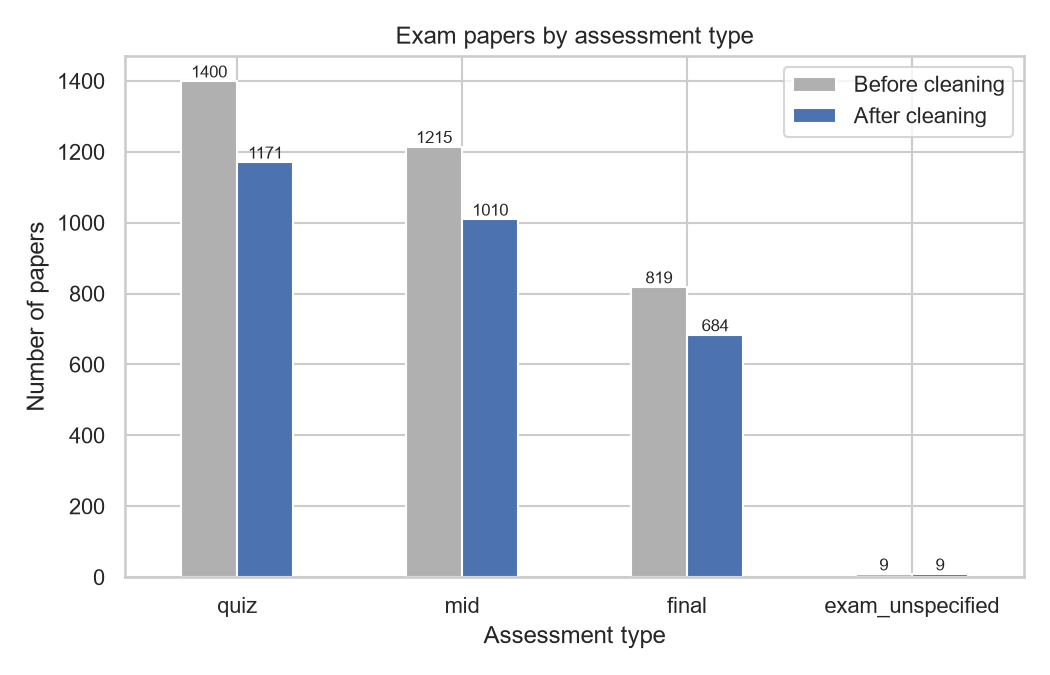
\includegraphics[width=0.78\linewidth]{01_papers_by_type.png}
\caption{Exam papers by assessment type, before and after cleaning (class distribution).}
\label{fig:class}
\end{figure}
Quizzes are the largest group (1{,}171 after cleaning), followed by mids (1{,}010) and finals (684); nine papers have no stated type. Cleaning removed a similar share of each type (about 16--17\%), so the balance between types was preserved.

\subsection{Subjects}
\begin{figure}[H]
\centering
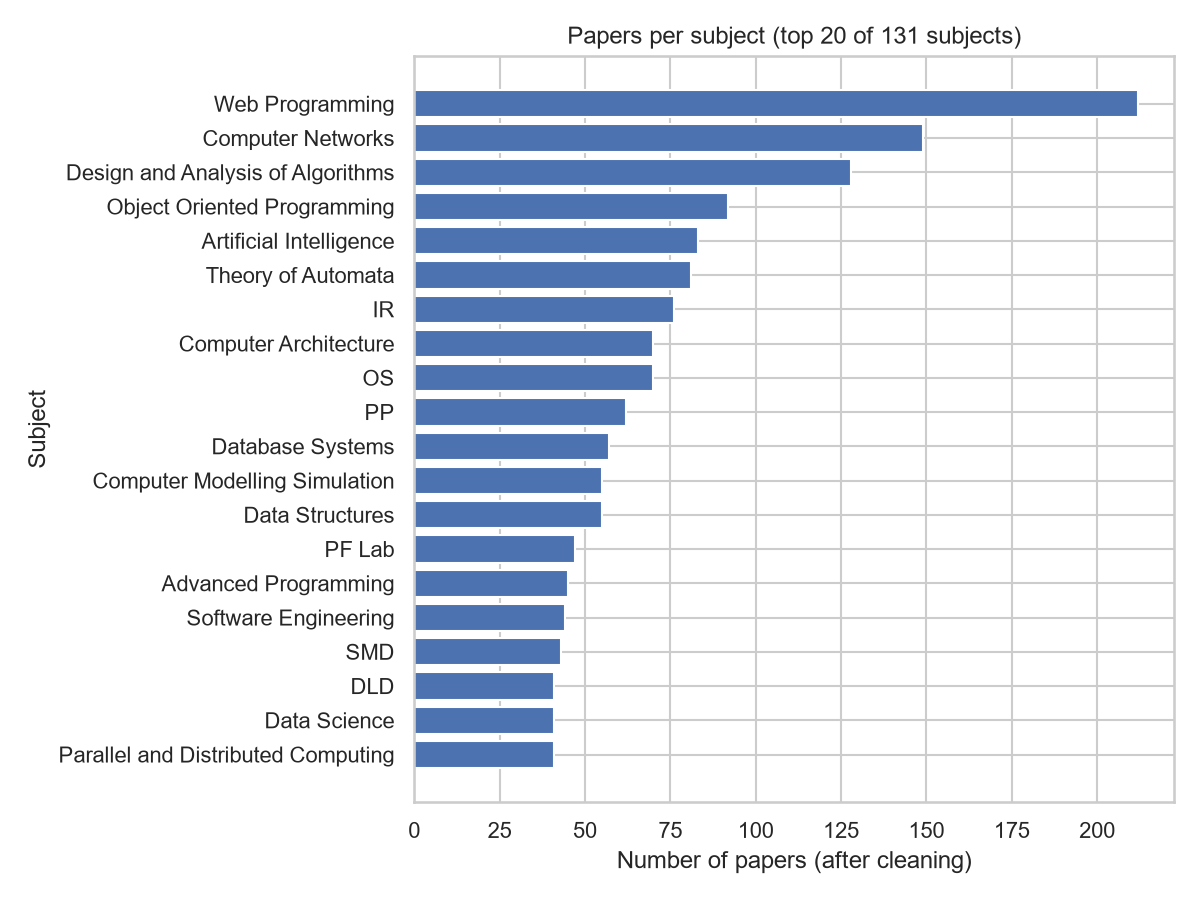
\includegraphics[width=0.78\linewidth]{02_papers_by_subject.png}
\caption{Papers per subject (top 20 of 131 subject labels).}
\end{figure}
The data is very uneven. The median subject has only 11 papers, and 31 subjects have fewer than five. The five largest subjects (Web Programming 212, Computer Networks 149, Design and Analysis of Algorithms 128, Object Oriented Programming 92, Artificial Intelligence 83) hold 664 papers, 23\% of the total. Pattern analysis will therefore only be reliable for well-covered subjects, and subjects with little history must be reported as low-confidence.

\subsection{Time Coverage}
\begin{figure}[H]
\centering
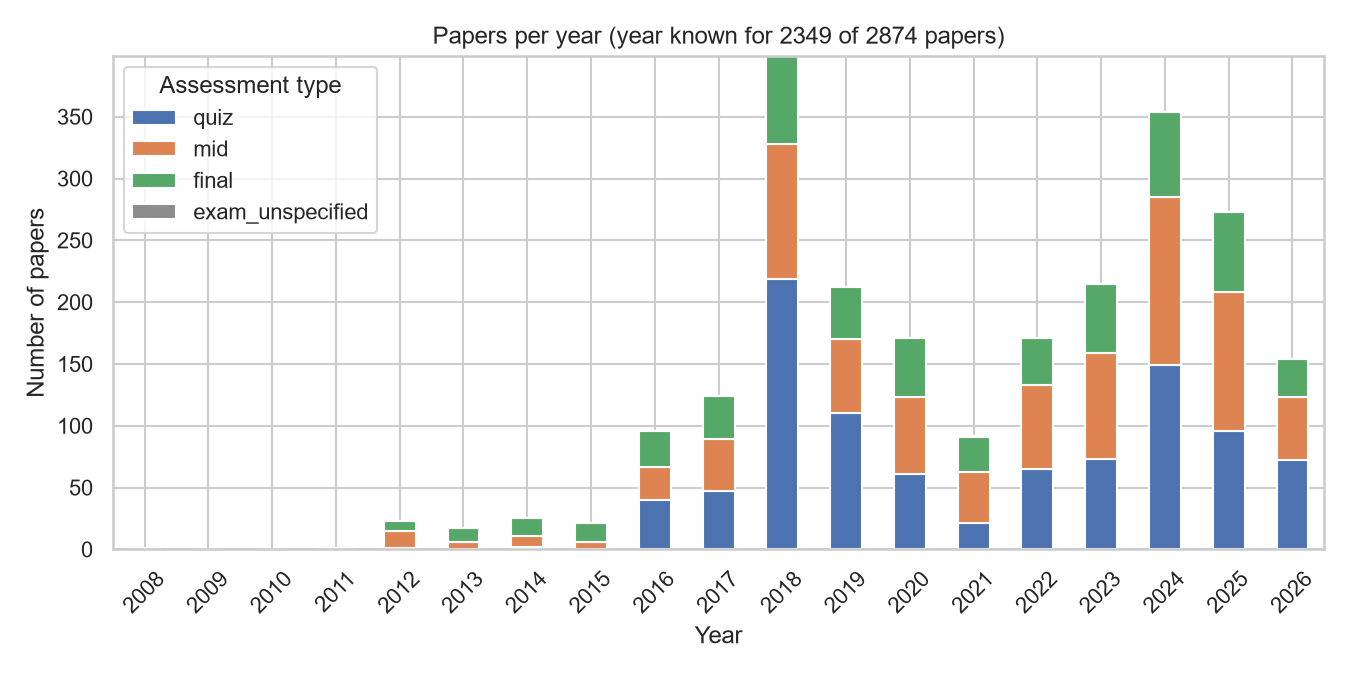
\includegraphics[width=0.9\linewidth]{03_papers_by_year.png}
\caption{Papers per year, stacked by assessment type (papers with a known year).}
\end{figure}
A year is known for 2{,}349 of 2{,}874 papers (82\%), spanning 2008 to 2026. The busiest years are 2018 (399 papers), 2024 (354) and 2025 (273). The data cannot tell us whether these peaks reflect more exams or simply more uploads by students. Fall (1{,}133) and Spring (1{,}020) are balanced, Summer has only 5 papers, and 716 papers have an unknown term.

\begin{figure}[H]
\centering
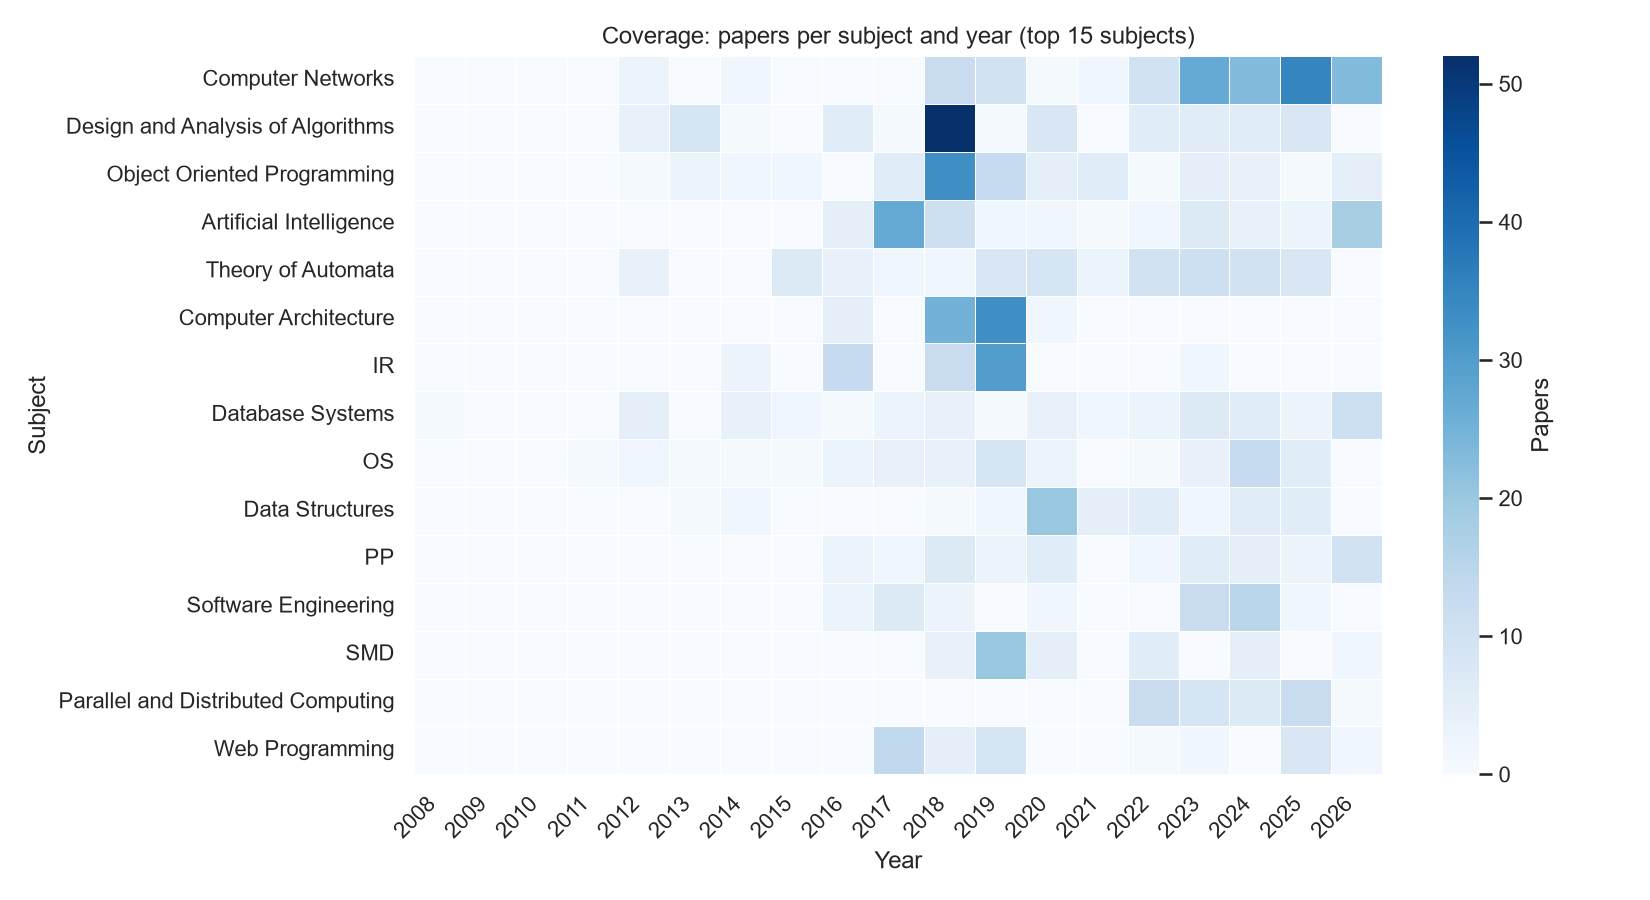
\includegraphics[width=0.95\linewidth]{04_subject_year_heatmap.png}
\caption{Coverage of the 15 best-covered subjects by year.}
\end{figure}
Even among the 15 best-covered subjects, 50\% of subject-year cells are empty. History is patchy, so a method that needs every year of a subject would not work on this data.

\subsection{Missing Data}
\begin{figure}[H]
\centering
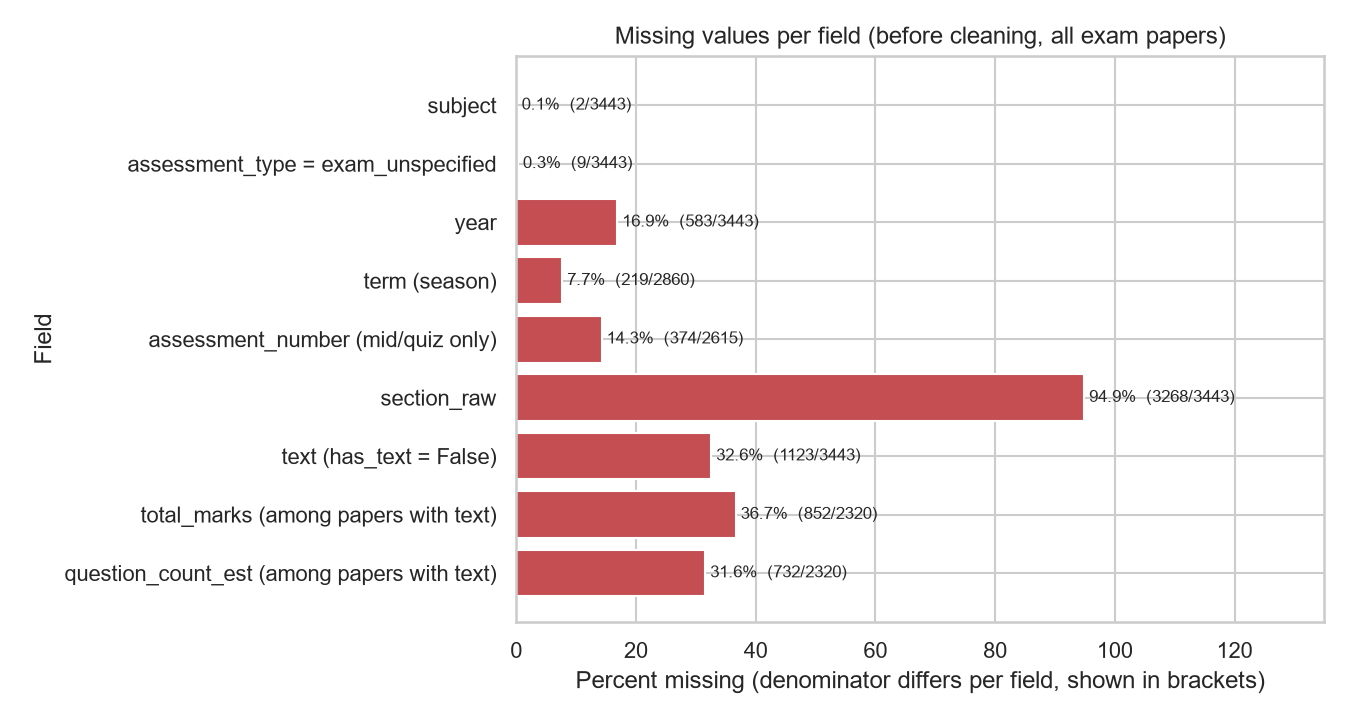
\includegraphics[width=0.9\linewidth]{05_missing_values.png}
\caption{Percentage of missing values per field before cleaning (denominators differ and are shown in brackets).}
\label{fig:missing}
\end{figure}
Year and readable text are the main gaps. Class section is missing for 94.9\% of papers, so it cannot support analysis at present. This also limits any attempt to separate patterns by section.

\subsection{Text Availability}
\begin{figure}[H]
\centering
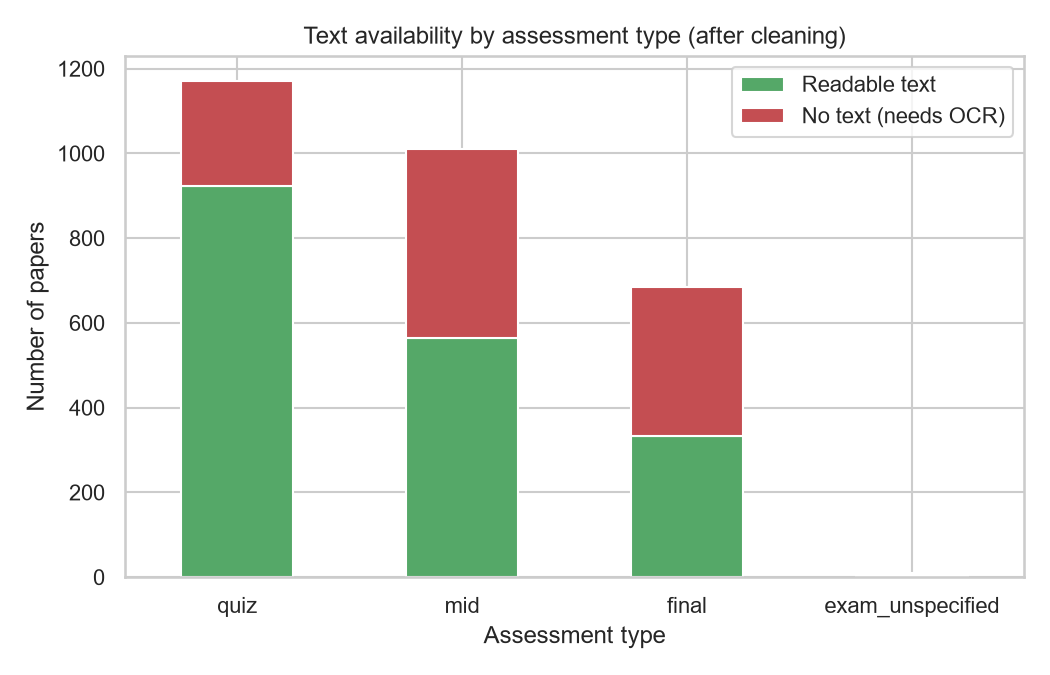
\includegraphics[width=0.78\linewidth]{06_text_coverage.png}
\caption{Papers with and without readable text, by assessment type.}
\end{figure}
Readable text is least available for the most informative papers: 21.2\% of quizzes, 44.2\% of mids and 51.5\% of finals have no readable text, and 24 of 130 subjects have no readable paper at all. This is the strongest argument for adding OCR in a later phase.

\subsection{Cleaning Effect}
\begin{figure}[H]
\centering
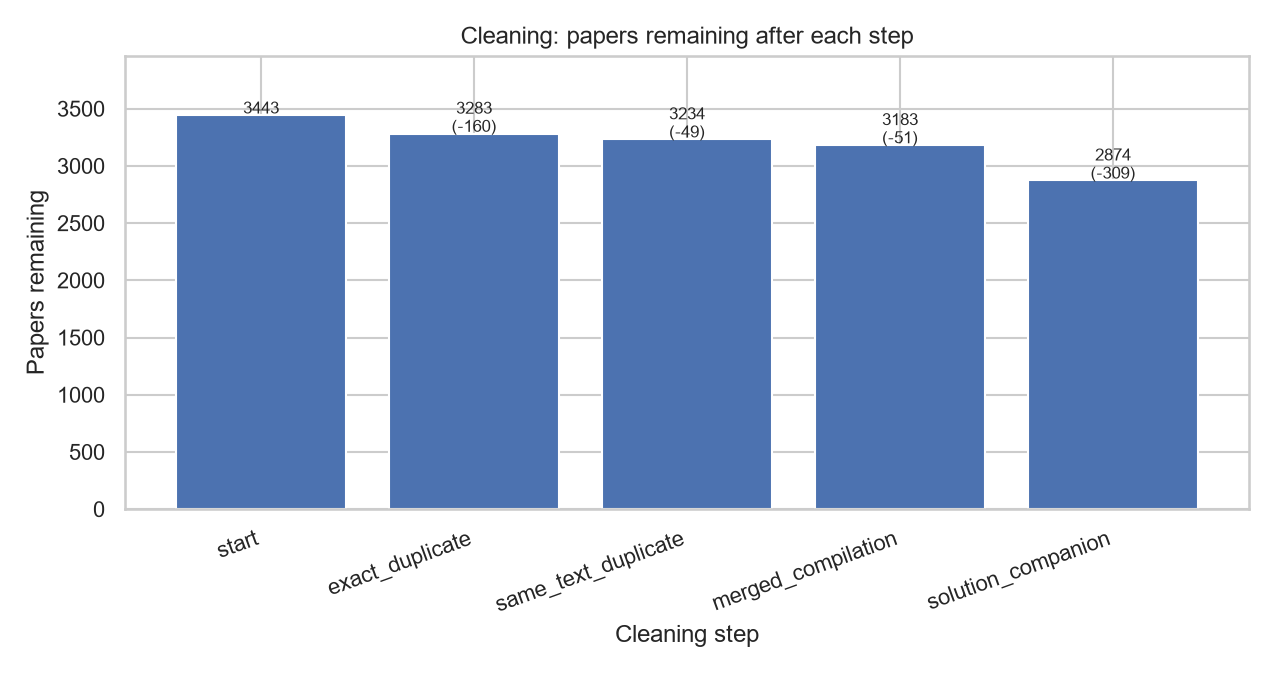
\includegraphics[width=0.85\linewidth]{07_cleaning_funnel.png}
\caption{Papers remaining after each cleaning step.}
\label{fig:funnel}
\end{figure}
Solution companions are the largest source of repetition (309 papers), followed by exact duplicates (160).

\subsection{Numeric Features by Assessment Type}
\begin{figure}[H]
\centering
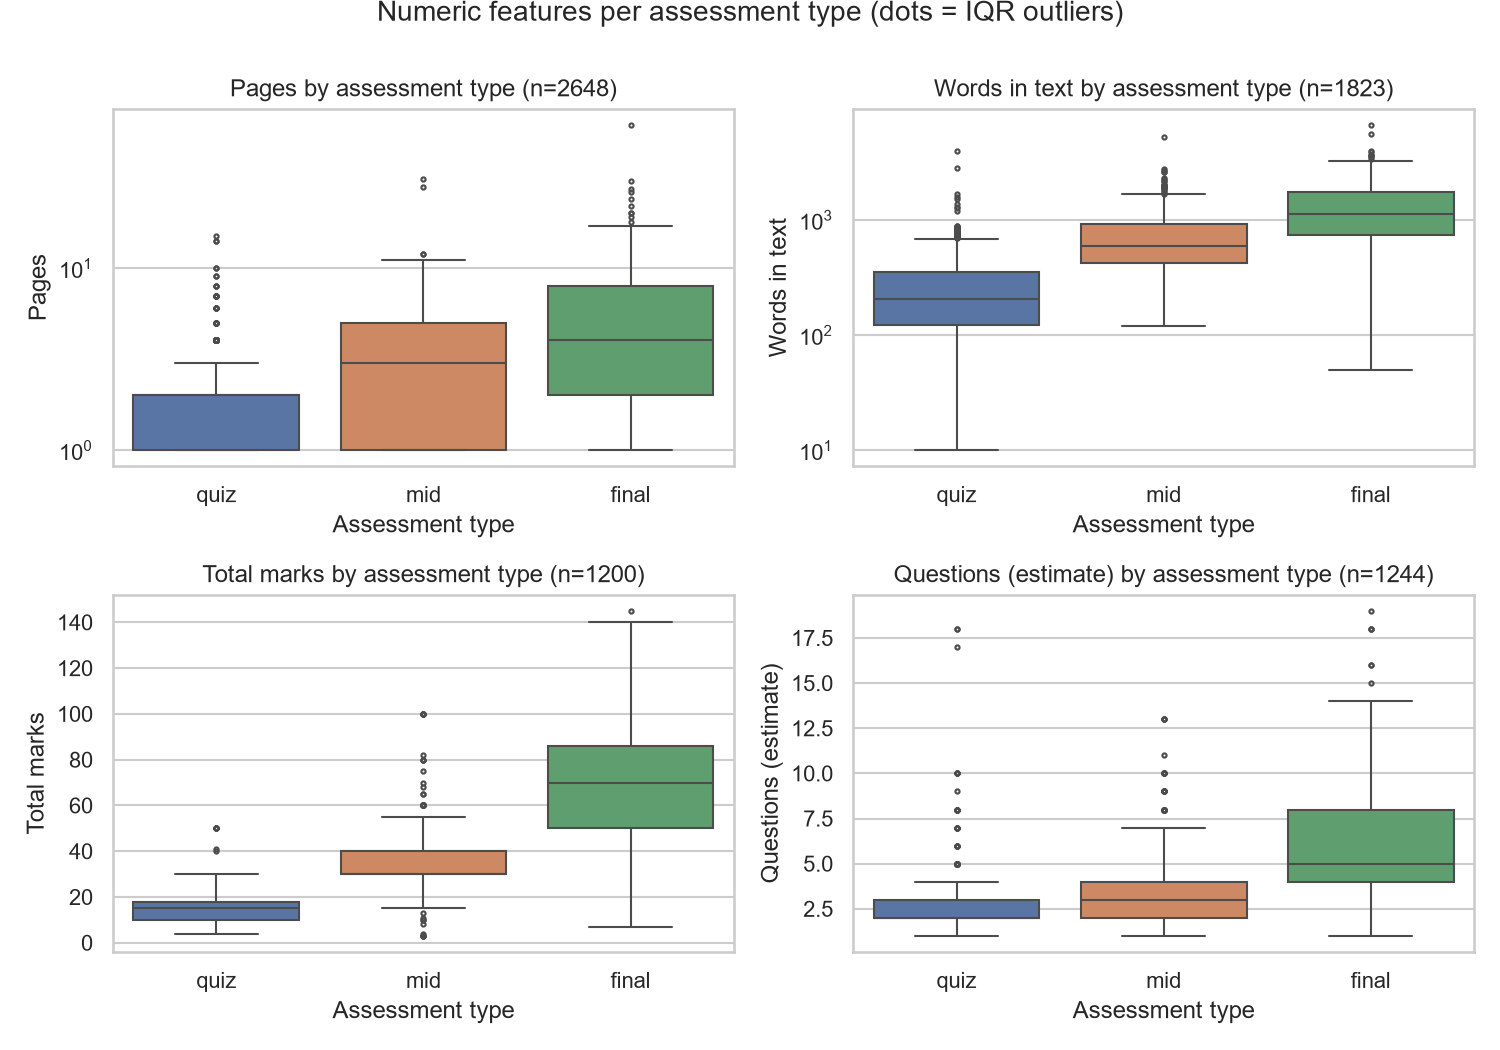
\includegraphics[width=0.95\linewidth]{08_numeric_boxplots.png}
\caption{Pages, words, total marks and estimated question count by assessment type (dots are IQR outliers; pages and words on a log scale).}
\end{figure}

\begin{table}[H]
\centering
\caption{Median values by assessment type (cleaned papers).}
\begin{tabular}{lrrrr}
\toprule
Type & Pages & Words & Total marks & Questions (est.) \\
\midrule
Quiz & 2 & 206 & 15 & 2 \\
Mid & 3 & 598 & 30 & 3 \\
Final & 4 & 1{,}126.5 & 70 & 5 \\
\bottomrule
\end{tabular}
\end{table}
Papers become steadily larger from quiz to mid to final on every measure. Assessment type is therefore a strong signal of a paper's shape, which supports the AI justification about assessment-specific patterns. (The nine unspecified papers are too few for a meaningful comparison.)

\subsection{Feature Correlations}
\begin{figure}[H]
\centering
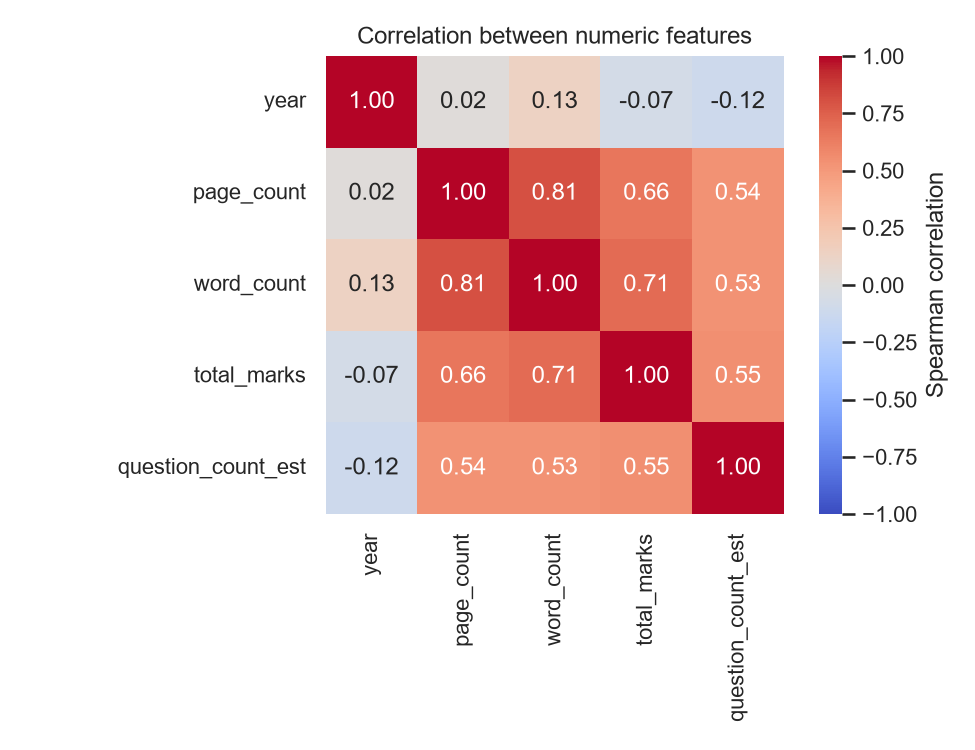
\includegraphics[width=0.62\linewidth]{09_correlation.png}
\caption{Spearman correlation between numeric features (pairs with both values present).}
\label{fig:corr}
\end{figure}
Paper size features are strongly related: pages and words ($\rho=0.81$), words and total marks (0.71), pages and total marks (0.66), and total marks and question count (0.55). Year is almost uncorrelated with the others (absolute values at most 0.13), so paper size does not appear to have changed much over time. Part of these correlations is caused by assessment type (finals are larger on every measure), and pages and words are measured from the same file; Phase~3 should consider dropping one of the redundant features.

%=====================================================================
\section{Limitations}
\label{sec:limits}
\begin{itemize}
  \item \textbf{One third of the papers are unreadable.} 32.6\% of exam papers have no extractable text (scans and photographs), mostly finals. Text-based analysis currently covers 1{,}823 of 2{,}874 clean papers, and 24 subjects have none.
  \item \textbf{Question-level data is not available yet.} Topics, difficulty and question types require NLP and are future work. Total marks and question counts are estimated with text patterns and are missing for roughly a third of readable papers.
  \item \textbf{Uneven coverage.} Half of the subjects have about 11 papers or fewer; many subject-year combinations are empty.
  \item \textbf{Metadata is parsed with rules.} Year, term, assessment type and number come from file paths and headers using regular expressions. We spot-checked samples while developing them, but we have not measured their accuracy on a manually labelled sample. 523 files with no assessment keyword were excluded and may include a few genuine papers.
  \item \textbf{Solutions may still repeat questions.} Solution files without a plain companion are kept and flagged.
  \item \textbf{Source quality.} The archive is student-contributed and may contain mislabelled or incomplete papers. Syllabi change over time, and course outlines in the archive come from different terms, so none can be assumed to be the current syllabus.
  \item \textbf{No professor-specific analysis.} The data contains no reliable instructor information for papers or quizzes.
  \item \textbf{Imputed values are placeholders.} Median-filled numeric features must not be treated as observed data.
\end{itemize}

\section{Future Work}
\begin{itemize}
  \item \textbf{Phase 3:} question-level extraction; topic and question-type labelling with NLP; frequency, recency and syllabus-relevance signals; probability model and tentative paper generation including lower-probability areas.
  \item \textbf{OCR} for scanned papers and photographs, starting with finals and subjects that currently have no readable papers.
  \item \textbf{Current syllabus:} allow a student to upload or select the current course outline and compare historical questions against it.
  \item \textbf{Personalisation and time management:} let a student attempt the generated paper under a time limit, analyse weak areas and speed, and generate a targeted follow-up paper.
  \item \textbf{Professor-specific quiz patterns} if a reliable quiz-to-instructor mapping becomes available.
  \item \textbf{Phases 4--6:} evaluation by historical backtesting with relevant metrics and bias checks, a hosted web application, and the final report.
\end{itemize}

\section{Conclusion}
Deliverable~1 defines the problem, audience and AI justification for SpillThePaper and builds a reproducible data foundation: 3{,}567 files collected from a pinned snapshot of a public archive, 3{,}443 structured exam-paper records, 2{,}874 papers after removing duplicates, flagged outliers, a documented feature strategy and nine exploratory charts. The analysis shows both the promise of the data (papers differ clearly by assessment type, and over a decade of history exists) and its main obstacles (a third of papers are unreadable without OCR, and coverage is uneven). These findings define the priorities for Phase~3.

\appendix
\section{Reproducing the Results}
After cloning the repository and installing the requirements in a virtual environment, run from the project root:
\begin{verbatim}
python "data scripts/01_discover.py"
python "data scripts/02_filter.py"
python "data scripts/03_download.py"
python "data scripts/04_extract.py"
python "data scripts/05_build_papers.py"
python "data scripts/06_clean.py"
python "data scripts/07_features.py"
python "data scripts/08_eda.py"
\end{verbatim}
Downloaded files are saved in \file{data/raw/} and extracted text in \file{data/interim/} (both excluded from Git). Small result tables are stored in \file{data/processed/}, charts in \file{eda/}, and execution logs in \file{logs/}.

\section{Repository Layout}
\label{app:repo}
\begin{verbatim}
SpillThePaper/
  README.md   .gitignore   requirements.txt
  config/          filter rules, assessment rules, subject name mapping
  data scripts/    all Phase 2 code (steps 01-08 and helper tools)
  data/processed/  small result tables (CSV) used as evidence
  eda/             exploratory charts (PNG)
  logs/            execution logs (collection, extraction, cleaning, EDA)
  report/          this report (LaTeX)
\end{verbatim}

\end{document}
